% (fold)
% Template: LaTeX file for ICMC 2010 papers, with hyper-references
%
% derived from the DAFx-06 templates
% derived from the ICMC 2009 templates by Steve Beck
%
% 1) Please compile using latex or pdflatex.
% 2) Please use figures in vectorial format (.pdf); .png or .jpg are working otherwise 
% 3) Please use the "papertitle" and "pdfauthor" commands defined below

%------------------------------------------------------------------------------------------
\documentclass[twoside,10pt]{article}
\usepackage{icmc2010,amssymb,amsmath} 
%\setcounter{page}{1}

\usepackage{listings}						% required for source code listings
\lstset{language=c++}
\lstset{basicstyle=\small\ttfamily}
\lstset{commentstyle=\color{commentcolor}}
\lstset{tabsize=2}
\lstset{gobble=2}							% eat the first tab in block listings
\lstset{aboveskip=\bigskipamount}			% amount of space above a block listing
\lstset{belowskip=\bigskipamount}			% ...

\usepackage{mathptmx} 

%____________________________________________________________
%  !  !  !  !  !  !  !  !  !  !  !  ! user defined variables  !  !  !  !  !  !  !  !  !  !  !  !  !  !
%==== set the title ====
\def\papertitle{A Flexible and Dynamic C++ Framework and Library for Digital Audio Signal Processing}
%\def\papertitle{}	%-- should be empty for the submission anyway!

%==== 1st submission: author name and affiliation are empty for anonymous submission ====
\def\paperauthorA{} 
\affiliation{}{}


%==== final submission: author name and affiliation ====
%---- uncomment 1 to 4 lines, for 1 to 4 authors
\def\paperauthorA{First Author}
\def\paperauthorB{Second Author}
\def\paperauthorC{Third Author}
\def\paperauthorD{Fourth Author}

%%---- set correspnding affiliation data for...
%%-- 1 author
%\affiliation{\paperauthorA}
%  {School\\ Department, City, Country \\ {\tt \href{mailto:email@domain.icmc}{email@domain.icmc}}}

%%-- 2 authors with same affiliation
%\affiliation{\paperauthorA, \paperauthorB}
%  {School\\ Department, City, Country \\ {\tt \href{mailto:email@domain.icmc}{email@domain.icmc}}}

%-- 2 authors with different affiliations
%\twoaffiliations{\paperauthorA}{School\\ Department}
%  {\paperauthorB}{Company\\ Address}

%%-- 3 authors with different affiliations
%\threeaffiliations{\paperauthorA}{School A\\ Department X}
%  {\paperauthorB}{Company\\ Address}
%  {\paperauthorC}{School B\\ Department Y}

%%-- 4 authors with different affiliations
%\fouraffiliations{\paperauthorA}{School A\\ Department X}
%  {\paperauthorB}{Company\\ Address}
%  {\paperauthorC}{School B\\ Department Y}
%  {\paperauthorD}{School C\\ Department Z}

%  ^  ^  ^  ^  ^  ^  ^  ^  ^  ^ user defined variables  ^  ^  ^  ^  ^  ^  ^  ^  ^  ^  ^  ^ 
%------------------------------------------------------------------------------------------

%%-- if using .ps or .eps figure files, they will be converted on the fly
%%-- RMK: for faster LaTeX runs, use it only once after adding new \includegraphics[]{} cmds
%\usepackage{epstopdf}	 

%---- the hyperref package must be last to properly work
\usepackage[pdftex,
       pdftitle={\papertitle},
	pdfauthor={\paperauthorA},
	colorlinks=false,bookmarksnumbered,pdfstartview=XYZ]{hyperref}
%\pdfcompresslevel=9
\usepackage[pdftex]{graphicx}	% for compatible graphics with hyperref
\usepackage[figure,table]{hypcap}	% corrects the hyper-anchor of figures/tables

% Stuff added by [tap]
\usepackage{hyperref}
\usepackage{url}
\usepackage{amsmath}
\usepackage{color}
\definecolor{black}{rgb}{0,0,0}
\hypersetup{colorlinks
,linkcolor=black
,filecolor=black
,urlcolor=black
,citecolor=black}
%reduces the space between the items in the itemize-environment 
\newenvironment{packed_item}{
\begin{itemize}
  \setlength{\itemsep}{1pt}
  \setlength{\parskip}{0pt}
  \setlength{\parsep}{0pt}
}{\end{itemize}}



\title{\papertitle}
% (end)

%------------------------------------------------------------------------------------------
\begin{document}

\DeclareGraphicsExtensions{.png,.jpg,.pdf} % used graphic file format for pdflatex
    
\maketitle

%%%%%%%%%%%%%%%%%%%%%%%%%%%%%%%%%%%%%%%%%%%%%%%%%%%%%%%%%%%%%%%%%%%%%%%%%%%%%%%%%%%%%%%%%%%

\begin{abstract}

This paper presents an object-oriented, reflective, light-weight application programming interface for C++, with an emphasis on real-time signal processing. It makes use of polymorphic typing, dynamic binding, and introspection to create a cross-platform environment pulling ideas from languages such as Smalltalk and Objective-C while remaining within the bounds of the portable and cross-platform C++ context.  The Jamoma Foundation and DSP Library provide a flexible framework and runtime environment, as well as an expanding collection of unit generators for synthesis, processing, and analysis.  This library has been used in both open source and commercial software projects over the past several years.

\end{abstract}


%%%%%%%%%%%%%%%%%%%%%%%%%%%%%%%%%%%%%%%%%%%%%%%%%%%%%%%%%%%%%%%%%%%%%%%%%%%%%%%%%%%%%%%%%%%

\section{Introduction} % (fold)
\label{sec:introduction}

``The SMC Roadmap identifies two broad research challenges: (1) To design better sound objects and environments and (2) To understand, model, and improve human interaction with sound and music.'' \cite{serra:2007}  The Jamoma Foundation and DSP Library directly addresses the first task as a means by which to address the second task.  Before discussing the approach and relative merits taken in the Jamoma project, we will first lay out some definitions and quickly review similar projects.


\subsection{Terminology} % (fold)

It is useful to clarify our usage of various computer science jargon and terminology.  In \emph{object-oriented programming} functionality related to a set of data is treated as a unit.  These units, or objects, are created and then often passed using a reference or pointer to the memory in which the object's contents are stored.  These objects comprise \emph{methods} (functions) and \emph{attributes} (properties or data which represent part of an object's state).

\textbf{Polymorphism} is a means by which a programming language generalizes different types of functions or data using a common \emph{API}, or Application Programming Interface.  An example of a polymorphic data-type of the variety in which we are interested is a `var' in the Javascript language\cite{Flanagan:2002}.  That is to say a data type which may be any data type internally (including an object or array), the details of which are not necessary in order to use or pass the data type amongst functions.

\textbf{Introspection} refers to the ability to determine the characteristics of an object at runtime.  This means that when handed a pointer in C++, we can take the pointer and query for an object's name, its type or \emph{class}, the messages that it understands, the attributes it possesses, etc.  By extension, \textbf{reflection} refers to the ability to then modify the behavior of an object at runtime\cite{Malenfant:1996}.  In practical terms this means adding messages, changing attributes, and extending existing instances of objects as the software is executing and without stopping the software to re-compile the code.

Introspection and reflection are often implemented by making use of a \textbf{dynamic binding model}.  Programming languages including C++ and Java link function and method calls when a program is compiled, known as static binding.  A dynamically bound model does not link these functions at compile-time, but instead waits until runtime to resolve the address of a method being called.  When a dynamic binding model is in use, calling methods is referred to as `sending messages' to objects.  Dynamic binding is the hallmark of languages such as Smalltalk, Objective-C, and Ruby.

Throughout the literature exists a confusing gaggle of terminology for classifying systems of objects.  These include \emph{framework}, \emph{library}, \emph{environment}, and \emph{toolkit}.  For the purposes of this paper, these will be defined as follows.  

\begin{packed_item}%\begin{itemize}
	\item unit generator 	: A class or object that implements a well-defined DSP task such as generating, analyzing, or processing audio data
	\item library        	: A collection of pre-built, ready-to-use, unit generators
	\item toolkit	     		: A collection of functions, utilities, and helpers, possibly with an API, for creating unit generators
	\item framework      	: An architectural structure that underlies a system of unit generators.
	\item runtime        	: A daemon or library operating in real-time when a framework, toolkit, or unit generator is in use.  A runtime's role is typically for dispatching messages, balancing processor loads, or otherwise running the background machinery such as in the Objective-C or Java runtime environments.
	\item environment    	: A full-fledged system intended for use by an end-user.  Examples include Max, SuperCollider, ChucK, DAW applications, and CSound.
\end{packed_item}%\end{itemize}

%(end)


\subsection{Requirements} % (fold)

The authors are involved in a number of divergent and parallel efforts requiring both a framework for creating unit generators and a library of ready-to-go unit generators.  These efforts include both open-source and closed-source commercial applications targeting multiple platforms and environments.  To meet the manifold demands of these endeavors the following list of requirements must be met regarding how said framework must perform and behave.

\begin{packed_item}%\begin{itemize}
	\item liberal licensing for both open source and commercial end use
	\item cross-platform (Mac/Windows/Linux/Embedded Devices/Mobile Platforms)	
	\item support for 64-bit audio signals
	\item multichannel audio support
	\item reasonably efficient (i.e. frame-based audio processing)
	\item user-extensible (adding functionalities without recompiling core frameworks)
	\item dynamically reconfigurable classes at runtime (dynamic-binding)
	\item process methods must be able to adapt to varying input (frame sizes, channel configurations, etc.) on-the-fly
	\item effortless to wrap (integrate?) classes for use in different environments (Max/MSP, VST, AU, ChucK, Pd)
%	\item be as thread-agnostic as possible (don't manage it, but take care of requisite protection, adaptable to various architectures) % new term: thread agnostic
%	\item MVC-friendly (reconfigurable) % new term: mvc

% TODO: Terms not defined: reconfigure classes, object decoration, process routine switching, frame-based audio processing, thread-agnostic, requisite protection,  MVC [tl]
% TODO: maybe simplify list, remove MVC?  [tap]

\end{packed_item}%\end{itemize}

Having met these technical requirements, the authors also deem an additional set of process requirements to be important.  These requirements are in adhering to contemporary philosophies for good coding practice, ensuring that it is pleasant to work with the code, to maintain it, to test it, and to distribute it.

\begin{packed_item}%\begin{itemize}
	\item expressive syntax, idioms, and conventions
	\item adhere to the DRY (Don't Repeat Yourself) principle, which states that ``Every piece of knowledge must have a single, unambiguous, authoritative representation within a system''\cite{Hunt:1999}
%	\item clear code % what do we mean by this?
	\item convention over configuration\footnote{\url{http://softwareengineering.vazexqi.com/files/pattern.html}}
	\item tag-based searching for class categorization and object instantiation
	\item integrated unit testing and benchmarking\footnote{\url{http://www.extremeprogramming.org/rules/unittests.html}}
\end{packed_item}%\end{itemize}

% One list for efficiency to the computer
% One list for efficiency for the development process / programmers's workflow : Ruby : set out top make a program that would "make programmers happy"; "Ruby is simple in appearance, but is very complex inside, just like our human body" - Yukihiro “matz” Matsumoto

% (end)
% (end)


%%%%%%%%%%%%%%%%%%%%%%%%%%%%%%%%%%%%%%%%%%%%%%%%%%%%%%%%%%%%%%%%%%%%%%%%%%%%%%%%%%%%%%%%%%%

\section{Prior Art} % (fold)
\label{sec:prior_art}

A myriad of existing libraries, toolkits, frameworks, and environments are available for digital signal processing.  To justify the effort of creating a new framework the merits of the extant members in this field should be considered, particularly with regard to our previously stated requirements.


\subsection{Choice of Language} % (fold)

An immediate winnowing of the field of contenders can be accomplished by discussing the choice of programming language.  There are popular and well structured DSP libraries for Java \cite{Guillemard:2005, Burk:1998} and Objective-C \cite{Jaffe:1989,Jaffe:1991}, for example, but these languages also carry restrictions and baggage.  Java is not installed on Windows systems by default and is not available in the context of many embedded devices.  Objective-C is available on Windows only through the clumsy and inadequate GnuStep\footnote{\url{http://www.gnustep.org/}} project\footnote{For example, one cannot natively compile using Microsoft's MSVC compiler.} and also is not available in the context of many embedded or mobile devices\footnote{The authors also look upon Apple's corporate control of the Objective-C language and runtime with some degree of skepticism, as compared to the open consortium that is mediating the C++ language's evolution}.  Interpreted languages such as Ruby and Python are quite powerful, but do not provide the required speed for real-time DSP performance in embedded environments and can also create portability problems in some cases. %TODO: is there any recent comparison of DSP speed between Java, Python and C ? [NP}  

Another class of languages are domain-specific languages for audio signal processing.  These include SuperCollider\cite{McCartney:1996}, ChucK\cite{wang:2008}, and CSound.  For our purposes we will also consider the Max family (including MSP\cite{Zicarelli:1998} and PureData\cite{Puckette:1996}) to be domain-specific-languages\footnote{We acknowledge the heated debate as to whether these environments actually constitute languages and the dispute regarding whether the use of these environments should be considered programming.}.  These domain-specific languages do provide facilities both for creating and using Unit Generators, but often have portability limitations and very frequently have licensing limitations\footnote{For example, ChucK and SuperCollider are licensed as GPL and thus not available for commercial development, while Max/MSP is not available on embedded devices nor in plug-in host environments other than Ableton Live}.  These environments also frequently have a large footprint in that they are very resource demanding, while we desire a light-weight framework.

The C++ language and its compilers are ubiquitous across platforms.  Plug-ins and extensions for sundry environments and languages can be compiled using C and C++.  The C++ language is also capable of creating extremely high-performance code optimized for digital signal processing.

% (end)


\subsection{Plug-in APIs} % (fold)

A related subject is the creation of audio plug-ins using existing APIs.  VST, RTAS, LADSSPA/DSSI, and AudioUnits are all APIs for creating UnitGenerators in C/C++.  None of these technologies, however, meet our requirements.  None are actually libraries, though there is a standard set of the non-cross-platform AudioUnit plug-ins provided by Apple.

% (end)


\subsection{Licensing} % (fold)

As stated, the authors require a framework that can be used in both open-source and commercial applications.  This immediately rules out the use of any existing work licensed under the GNU GPL, which stipulates that all works using it are themselves licensed under the GNU GPL.  Among the options this rules out are SndObj\cite{Lazzarini:2001}, CLAM\cite{Amatraian:2008}, and Marsyas \cite{Tzanetakis:2008}.  Additionally, the CSL framework\cite{Pope:2003} requires licensing through the University of California, which is not agreeable to the open use we require.

Due to these licensing restrictions, none of these packages are suitable for our use\footnote{The license for the STK is reasonably liberal.  At the time that the Jamoma DSP library was initially written, however, the license for the STK specified non-commercial use and thus using the STK was not an option for the authors.}.  They do, however, contain many valuable ideas that serve to inform our own work.

% (end)


\subsection{Dynamic Binding} % (fold)

One of our core concerns is the requirement for dynamically reconfigurable classes at runtime.  For this, dynamic binding is of critical importance.  Dynamic binding is implemented to some degree in many of the aforementioned environments including Marsyas, Max/MSP, and the NeXT SoundKit for Objective-C.  However, due to our cross-platform and liberal licensing requirements they are not options.  Of the remaining DSP libraries and toolkits, the STK\cite{Cook:1999}, CMix\cite{Lansky:1990}, and TANGA\cite{Reiter:2007} are all statically-bound.  

An interesting middle-of-the-road option is Kronos.  In fact, the problem domain of the Kronos system is the same as our problem domain: `` the musician may want to change the program during its execution. This was possible in the analog music studio, where swapping out patch cords often resulted in immediate gratification. In the digital world programs often have to be aborted, edited, re- compiled, linked and launched. The all-important musical hacking suffers from such a heavy compilation cycle, making a traditional programming language less desirable for real time artistic expression.'' \cite{Norilo:2009}

Dynamically-bound frameworks and runtimes, such as PureData, Objective-C, or Marsyas, solve this problem by precompiling the unit generators and then directing messages to these objects at runtime.  Kronos takes an alternative approach where the graph of objects, indeed the unit generators themselves, are not precompiled at all but rather compiled `Just in Time' from a custom meta-language. This results in better performance from the code, while still maintaining much of the flexibility offered by a dynamically-bound runtime.  The performance results are compelling.  Unfortunately a just-in-time compilation still requires compilation every time you change the interconnections between objects, and the resulting domain-specific language may be limited to only the domain for which it is written.

% (end)


\subsection{ZenGarden} % (fold)

Having narrowed the field to libraries and toolkits with suitable (or potentially suitable) licensing and platform independence, and also built on a dynamically-bound architecture, we are left with only one package that is readily available: ZenGarden\footnote{\url{http://github.com/mhroth/ZenGarden}}.  ZenGarden is a dynamically-bound cross-platform framework licensed under the LGPL.  PureData can be used as an authoring environment to define a graph of ZenGarden's unit generators, as was done for the popular RjDj iPhone app\footnote{\url{http://rjdj.me/}}.

While ZenGarden has much to offer, it still lacks out-of-the-box support for 64-bit audio processing graphs and the kind of dynamic multichannel audio operation that is required.

% (end)


\subsection{Conclusion} % (fold)

In the end we found no one framework to possess all of the requirements set forth.  As the de facto standard for audio DSP libraries, the STK comes perilously close as of more recent revisions\cite{Scavone:2005}, and offers a rich and mature array of unit generators.  The STK is statically-bound.  While a problem for the kinds of applications we envision, this does yield potentially faster execution of the code.  We propose an alternative that will not replace the STK, but rather coexist with it as a part of the greater computer music ecology.

% Why in the world do we need another DSP framework?

% TODO: Section 5 of Amatraian:2008 maybe provide the start of a way to categorize different frameworks.
% I'm not sure if it actually makes sense to distinguish between text and gui interfaces, given that the 
% underlying data-flow basis is exactly the same (as argued in several of the Tzanetakis papers)  
%
% However, I think it is useful to distinguish between Unit Generators (STK, AU, VST), Unit Graphs
% (AUGraph, Multicore, ?), and those that combine both into one (CLAM, Max/MSP, Marsyas)
% [tap]

% (end)

% (end) section:Prior Art



%%%%%%%%%%%%%%%%%%%%%%%%%%%%%%%%%%%%%%%%%%%%%%%%%%%%%%%%%%%%%%%%%%%%%%%%%%%%%%%%%%%%%%%%%%%

\section{The Jamoma Platform} % (fold)

Jamoma was initially conceived as a modular standard for structuring patchers in Max \cite{Place:2006}. Over the last few years, however, it has been greatly augmented.  Jamoma has now developed into a platform providing a layered architecture of frameworks that combine to provide essential functionality for creating computer music systems in general, not just for Max/MSP.

\begin{figure}[htbp]
\centerline{\framebox{
	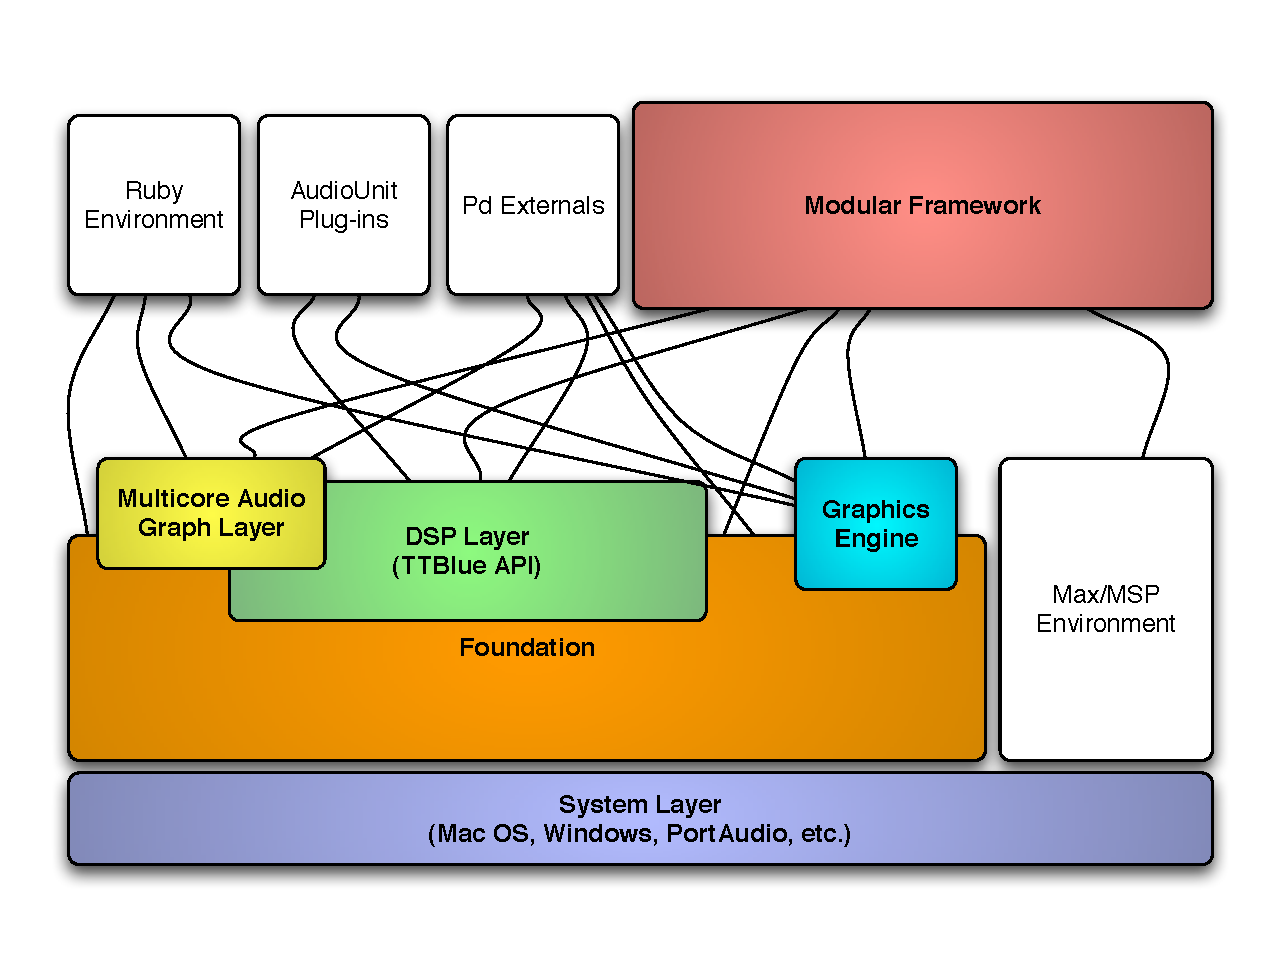
\includegraphics[width=0.9\columnwidth]{layers}}}
\caption{The Jamoma Platform as Layered Architecture.}
\label{fig:layers}
\end{figure}

In this layered architecture frameworks may build upon and extend frameworks below them in the hierarchy, but the lower frameworks have no knowledge of the higher frameworks.  Divisions between the frameworks help to establish clarity as to what functionalities belong to which part of the system.  Users of Jamoma may then use only the parts of the system that are relevant to a given project.  The Jamoma Platform currently consists of five frameworks: Jamoma Foundation, Jamoma DSP, Jamoma Multicore, Jamoma Graphics and Jamoma Modular. This paper is focusing on the Jamoma Foundation and Jamoma DSP frameworks. Figure~\ref{fig:layers} illustrates the layers of the Jamoma Platform.  Each colored shape is implemented as it's own framework.

Each framework within the Jamoma Platform shares a common structure.  A shared-library implementing base classes and core functionality exists at the core.  This functionality is then extended and enhanced by creating extensions.  An extension is a plug-in library that is dynamically loaded at runtime.  In this way the system can be expanded without re-compiling core components.

% The Jamoma Platform is not an environment.  It is a set of frameworks that can be used to create environments, or to extend existing environments, but it is not itself and environment. 

This layered approach is similar to other such approaches in the field including its application by the authors to spatialization systems\cite{Peters:2009}.


\subsection{Foundation} % (fold)

The Jamoma Foundation\footnote{\url{http://github.com/tap/JamomaFoundation}} may be seen as analogous to the Objective-C Foundation, which ``Defines the `nuts and bolts' classes for Objective-C programming''\footnote{\url{http://developer.apple.com/cocoa/}}.  The Jamoma Foundation defines base classes, including our primary base class, \texttt{TTObject}.  Object life-cycle facilities include factories for creating, destroying, and referencing these classes.  A message-passing and attribute system inspired by Smalltalk\cite{Krasner:1988} and Objective-C\cite{Cox:1986} is implemented to enable dynamically-bound object topologies.  

The Jamoma Foundation classes are informed by many best-practices of software development.  Unit Testing, for example, is integrated directly into the class design.  There is also an emphasis on the use of design patterns\cite{Gamma:1995}.  In particular, all objects possess a built-in observer notification system.  

As much as possible, complexity, `glue code', and the mechanics of writing C++ are hidden from the programmer.  They may be accessed if necessary, however, by relying on a convention-over-configuration paradigm the clarity of the code is dramatically improved.  In the opinions of the authors' this makes the code not only less time consuming to create and maintain, but also more enjoyable.  This aim is also aided by emphasizing DRY principles throughout the Jamoma Platform.

Functionality specific to audio or digital signal processing is not present in this particular framework.  In fact, the Jamoma Foundation can be used as a general framework and runtime as a dynamically-bound API layer on top of C++ for any purpose.  This is evident, for example, in the Jamoma Graphics Library.

\subsubsection{Messages and Attributes} % (fold)

As with other similar runtime systems, the Jamoma Foundation defines a symbol table for efficient message dispatch and lookup.  This symbol table is leveraged in the implementation of messages and attributes.  

A \emph{message} is defined as a method of a class or instance that is then bound to a symbol.  Messages may optionally possess arguments for passing data to and from the object.

An \emph{attribute} is defined as a data member of a class or instance, whose access is bound to symbol.  Typically, the setting or retrieving of the value then uses a built-in accessor method.  If needed, a custom setter or getter method can be defined to override the built-in mechanism.

Additionally, attributes may possess \emph{properties}.  Properties are implemented as attributes of the attribute.  They include the ability define ranges for an attribute, the behavior of an attribute's value when the range is exceeded, etc.  The design of this system is consistent with the authors' previous proposals for more sophisticated control in parametric systems\cite{Place:2008params}.

% (end)
% (end)


\subsection{DSP Layer} % (fold)

The Jamoma DSP Layer\footnote{\url{http://github.com/tap/JamomaDSP}} augments the Foundation by extending \texttt{TTObject} to create a new \texttt{TTAudioObject} base class.  \texttt{TTAudioObject} provides the core functionality for processing multichannel, 64-bit, audio samples singly or in blocks while providing basic thread protection.  It also provides attributes and audio processing methods for controlling muting, bypass, sample-rate, etc. which are inherited by subclasses.

In addition to the framework and base-classes, the DSP player also provides toolkit functionality with convenience functions such as denormals and dc-offset blocking, and a library of classes as extensions implementing a variety of unit generators.  The provided unit generators include basic trigonometry functions, filters (including butterworth), oscillators, noise generators, analysis, effects, etc.

% (end)


\subsection{Additional Layers} % (fold)

Additional layers have been implemented on top of the Jamoma Foundation, both in series and in parallel with the DSP layer.  For example, a \emph{Graphics Layer}\footnote{\url{http://github.com/tap/JamomaGraphics}} based on Cairo\footnote{\url{http://cairographics.org}} provides both a platform-independent, and a host-independent, way to draw to the screen.  While not necessarily related to audio or DSP it is relevant in that GUI widgets can be created that will work, for example, both in the Max/MSP environment and in an AudioUnit plug-in.

Many of the initiatives reviewed in Section~\ref{sec:prior_art} combined not only a means by which to create unit generators, but also a method by which unit generators are combined into a graph for processing audio.  In the Jamoma Platform we create a clear division between creating and using unit generators versus combining them into a graph.  This allows the unit generators to be combined in any way that seems desirable for a particular context.  The \emph{Jamoma Multicore Audio Graph Layer}\footnote{\url{http://github.com/tap/JamomaMulticore}} is a framework that manages the creation of graphs of \texttt{TTAudioObject} instances.

Jamoma Modular\footnote{\url{http://github.com/tap/JamomaModular}} is a modular framework for a structured approach to development and control of modules in the Max/MSP/Jitter environment.  It builds upon the Foundation, DSP, Graphics, and Multicore frameworks to accomplish this end.

% (end)


\subsection{Ruby Language Bindings} % (fold)

As a dynamically-bound API, the Jamoma Foundation is a natural fit for control from the Ruby environment.  Language bindings for Jamoma in Ruby exist via the Jamoma Ruby project\footnote{\url{http://github.com/tap/JamomaRuby}}.  This enables use in a wide range of applications including live coding using \emph{irb}\footnote{\url{http://ruby-doc.org/docs/ProgrammingRuby/html/irb.html}} and integration with web applications using \emph{Ruby on Rails}\footnote{\url{http://rubyonrails.org}}.

% (end)
% (end)


%%%%%%%%%%%%%%%%%%%%%%%%%%%%%%%%%%%%%%%%%%%%%%%%%%%%%%%%%%%%%%%%%%%%%%%%%%%%%%%%%%%%%%%%%%%

\section{In Practice} % (fold)

\subsection{Applications}

The technical underpinnings of the Jamoma Foundation and DSP Library lend themselves to a variety of applications.  The API provides a clear interface to both creating and using unit generators in the C++ language or Ruby.  Additional tools and facilities have been fabricated to make Jamoma DSP's unit generators readily available in several popular environments.


\subsubsection{Max/MSP}

Given a Jamoma DSP unit generator, this object can be easily compiled for Cycling '74's Max/MSP environment.  One method for accomplishing this is to use the Jamoma DSP ``Class Wrapper'', which takes an existing class and creates bindings for the target environment.  Following, is the complete code listing for an N-channel MSP external that wraps the Jamoma DSP limiter class.

\begin{lstlisting}
    #include "TTClassWrapperMax.h"
    int main(void)
    {
        TTDSPInit();
        return wrapTTClassAsMaxClass(TT("limiter"), "myMaxLimiter~", NULL);
    }
%\end{lstlisting}

In addition to simply wrapping existing classes for MSP, it is possible to use the Jamoma DSP objects in other ways.  One example is the \texttt{jcom.filter~} external provided with Jamoma DSP.  This object dynamically loads any of a variety of filter classes from the DSP Library.  The classes are loaded and swapped on-the-fly, without requiring Max's DSP chain to be rebuilt.  The code for the \texttt{jcom.filter~} object searches the object registry for available filter classes to present a list of choices for the user.  This list will then be dynamically updated if new filters are added without requiring any code to be compiled or updated.


\subsubsection{Plug-ins}

Jamoma DSP includes a number of example projects that include VST and AudioUnit plug-ins.  AudioUnit plug-ins requiring only a generic interface may be created using a class wrapper similar to the one for creating Max/MSP externals.  

The ViMic project is (TODO: Nils, we need a one sentence description).  In the summer of 2009 Vimic was implemented as an AudioUnit plug-in, using elements of the Jamoma Platform.  The signal processing is handled using Jamoma DSP and a custom UI is realized by employing the Jamoma Graphics Library.  See the screenshot (TODO: Nils -- screenshot). 


\subsubsection{Ruby, IRB, Rails}

Ruby Language Bindings make the entirety of the DSP library accessible in the Ruby environment.  Together with Jamoma Multicore, Ruby's interactive shell (irb) can be use for live-coding by creating objects and manipulating the graph of those objects in real-time.  The following code shows a much simpler irb session. This creates an instance of a lowpass filter and then passes some values one-at-a-time through the filter.

\begin{lstlisting}
    $ irb
    >> require 'TTRuby'
    JamomaFoundation -- Version 0.6
    JamomaDSP -- Version 0.6
    => true
    >> f = TTRuby.new("lowpass")
    => #<TTRuby:0x1011db170>
    >> f.calculate(1.0)
    => 0.25
    >> f.calculate(1.0)
    => 0.4375
%\end{lstlisting}


\subsubsection{Additional Environments}

Jamoma DSP includes further example projects wrapping classes for PureData and SuperCollider.



- Applications
[TL]    - DBAP interesting example of what kind of units Jamoma DSP can cater for
        - split personality operating at audio and control rate
            - two units tied together at runtime
                - audio matrix
                - coefficients for matrix calculated at control rate
        - a biquad filter is really the same ....
            - but if values at control rate can cause interpolation to new value, the ramp lib could get involved and we could choose what curve to use for interpolation (e.g. glissandi in the pitch domain)

\section{Discussion}

% TODO: How do we explain this in 15 minutes so that it seems significant to someone new?
% _How_ do we go ahead to implement the fancy stuff that we required? Are there important design decisions involved that are worth presenting/discussing?
% What's Cool:
%   1. writing unit generators is clear and straight-forward (e.g. gain, delay, \ldots)  -- thanks in part to convention over configuration, DRY,...
%   2. combining unit generators is simple - example: combining simple units into compound (e.g. DC Blocker: see Section 'Examples')
%   3. wrapping for different environments is easy - this will be further improved in future using Jamoma Graphics

The GNU LGPL license chosen for the Jamoma frameworks have enabled them to be used for open-source as well as commersial software development: 

Electrotap's Tap.Tools\footnote{http://shop.electrotap.com/products/taptools} is ashareware collection of 3rd party externals for Max/MSP. Tap.tools have a particular emphasis on common audio effects processing, and inherits multichannel audio support and 64-bit internal processing from the Jamoma DSP library.

Jamoma Modular \cite{Place:2006} is a framework providing a structured approach to development and control of modules in Max/MSP, licensed as GNU LGPL. Several 3rd party libraries of Jamoma Modules are currently in developmeent. The license used for Jamoma Modular allows such libraries to be made available on a commercial basis as well as open-sourced.

The now discontinued Hipno\cite{Place:2005} was a set of audio effects plug-ins available as VST, RTAS and Audio Unit. Hipno plug-ins were developed in Max/MSP using Tap.tools and Jamoma DSP functionalities, and used the now dicontinued Cycling'74 Pluggo environment for plug-in wrapping. The cross-platform requirement detailed earlier has enabled Tap.tools, Hipno and Jamoma Modular to be developed for Mac OSX as well as Windows. One of the aims of Jamoma Graphics framework is to provide the structural framework for development of units with graphical user interfaces that can be wrapped as externals for environments such as Max, Pd and SuperCollider as well as being turned into plug-ins, independent of external wrapping environments such as the now dicontinued Pluggo.


    Benefits:
        % - available for open and commercial products - used for Jamoma Modular, Hipno, TapTools, ... - DONE
        %- cross-platform - Jamoma available for Max and Windows - DONE
        - "effortless to wrap" -  provide example of code for Max external, screenshots of external in Max, AudioUnit,...
        - user-extensible - function lib, analysis lib, math lib, 
        - reuse of code in different environments: (going beyond flext) but more pleasant
        - dynamically reconfigurable objects without recompiling code or DSP graphs
            - FM example
            - Live coding (irb?)
        - multichannel, adapt to varying input  - quote the not net written paper for DAFx
        - 64-bit - higher fidelity, timing issues when counting samples, better use of modern processors
        - thread-agnostic
        - "code pleasant to work with"
        - Introspection features of the Jamoma Foundation make it possible to query objects to automate the process of creating mappings and advanced control of the objects such as those cataloged in [18].
        - Because we can put together objects in the environment of our choice: Max, Pd, a DAW if we use AudioUnits, and then even a web-browser using Ruby on Rails. Then we can move the code from one environment to another easily, or port it back to C++ with minimal effort.

    Downsides (if any):
        -  dynamically binding is not as fast
        - 
    
- Future work (no subsections -- the headers waste space)

    - Graphics
    - Multicore
    - Server-side web application framework. :-)
    - SuperCollider wrapper
    - Scheduler - possibilities for sample-accurate scheduler?
    - Processing arrays
    - Node Lib
    - Web Browser Support
    - more units, support for common and well-established audio processing methods -  is it possible to borrow code from other projects where license permits it?
    - 
    

    
% (end)
    

%%%%%%%%% OLD STUFF FROM HERE ON



%%%%%%%%%%%%%%%%%%%%%%%%%%%%%%%%%%%%%%%%%%%%%%%%%%%%%%%%%%%%%%%%%%%%%%%%%%%%%%%%%%%%%%%%%%%

\section{Examples} % (fold)

1. DC Blocker class

2. How to wrap the class

3. How to combine two classes: e.g. noise + bandpass filter

4. FM that can be repatching the FM unit in real time (different algorithms)  -- (perhaps this could a part of the discussion section?) 

%TODO: Trond will try to find examples/graphics illustrating this for further discussions between authors
% I would guess more here than in the multicore, as it's an example of dynamic binding between units


%TODO: interpolation for TTWavetable

%TODO: Non-linear filters - limiting or saturation inside the filter as xn is cast to xn-1 and yn to yn-1 (switching the feedback-filter on the fly)

% (end)


%%%%%%%%%%%%%%%%%%%%%%%%%%%%%%%%%%%%%%%%%%%%%%%%%%%%%%%%%%%%%%%%%%%%%%%%%%%%%%%%%%%%%%%%%%%

\section{Discussion / Applications} % (fold)

Real-world usage...

\subsection{Spatialization}

%TODO: CUT THIS:
%Spatialization at the Encoding/Decoding and Authoring layers\cite{Peters:2009}.  In fact, through the development of the NodeLib we are now able to work also at the Scene Description Layer by communicating as SpatDIF\cite{Peters:2008spatdif}.

One example that is ready for implementation in the Jamoma DSP library is DBAP\cite{Lossius:2009}.


\subsection{AudioUnit Creation}

In the summer of 2009 we combined the application domains of spatialization, graphical rendering, and AudioUnit creation to create a plug-in version of ViMiC\cite{Peters:2008b}.

% TODO: Nils, do you have a a screenshot we could add here?  [tap]


\subsection{External Object Generation for Max/MSP and PureData}

Class wrappers...  What about SuperCollider?  I guess we should actually do it first before we claim that we can.

Electrotap's Tap.Tools\footnote{http://electrotap.com/taptools}

Cycling '74's Hipno\cite{Place:2005}

Jamoma Modular Framework\cite{Place:2006}


\subsection{Ruby and Ruby on Rails}

Server-side web application framework.  :-)

\subsection{Rapid Prototyping Environment}

Because we can put together objects in the environment of our choice: Max, Pd, a DAW if we use AudioUnits, and then even a web-browser using Ruby on Rails.  Then we can move the code from one environment to another easily, or port it back to C++ with minimal effort.

\subsection{Mapping}

Introspection features of the Jamoma Foundation make it possible to query objects to automate the process of creating mappings and advanced control of the objects such as those cataloged in \cite{Pendharkar:2006}.  


% (end)

%%%%%%%%%%%%%%%%%%%%%%%%%%%%%%%%%%%%%%%%%%%%%%%%%%%%%%%%%%%%%%%%%%%%%%%%%%%%%%%%%%%%%%%%%%%

\section{Further Development} % (fold)


\subsection{ClassWrappers}

For more environments, such as VST and SuperCollider

\subsection{DSP Library Expansion}

Spectral processing \\

Granular processing   \\

More effects (reverb, pitch-shifting, chorus) 


Spectral(FFT) Processes\\

SynthesisLib

\subsection{Scheduler}

Initial work on a scheduler for the DSP library was begun in 2007.  Competing priorities have left it unfinished...  More interesting models for scheduling, such as the the model implemented in ChucK provide impetus for further research into new approaches to this topic.


\subsection{Web Browser Support}
We have begun implementing support for server-side integration of the Jamoma Runtime via the Ruby language bindings and Ruby on Rails\footnote{http://rubyonrails.org}.  To fully leverage the DSP library and Jamoma Foundation in a web-browser we need the ability to invoke the runtime on the client-side of the equation through a web browser plug-in similar to that done in the iARS Project\cite{Frauenberger:2003}.


\subsection{NodeLib}

As a means of addressing parts of the system via OSC.  Somewhat like what Marsyas does.  An implementation of the ideas presented in\cite{Place:2008osc}.


\subsection{Processing Arrays}

[12/10/09 7:58:39 PM] Nils Peters: on the other hand, IMHO in most use cases you want to have separate control over the filter parameter of each channel

[12/10/09 8:00:26 PM] Nils Peters: or the delay

[12/10/09 8:00:41 PM] Nils Peters: You want to set different delays to your input channels

[12/10/09 7:59:32 PM] Tim Place: It could be possible to create an object which wraps an array of objects that process each channel individually

[12/10/09 7:59:58 PM] Tim Place: I think that would address the filter problem you mention more generally



% (end)

%%%%%%%%%%%%%%%%%%%%%%%%%%%%%%%%%%%%%%%%%%%%%%%%%%%%%%%%%%%%%%%%%%%%%%%%%%%%%%%%%%%%%%%%%%%

\section{Summary} % (fold)

Jamoma Foundation and DSP provide a flexible, user-extendable, runtime environment for creating and using audio and digital signal processing objects.  Due to its advanced use of dynamic binding and message-passing paradigm, the building blocks can be reconfigured at runtime without requiring re-compilation, but with the unit generators themselves compiled as C++ and performing block-processing we retain the performance of a compiled language.


"A well-defined API can also speed up the development process, since the implementation can focus more on the algorithmic aspects and less on implementation issues like API design." \cite{Lerch:2005}

The power of this runtime is demonstrated through the ability to compile objects for Max, Pd, AudioUnits, VST, etc.  The future includes Multicore.

% (end)

%%%%%%%%%%%%%%%%%%%%%%%%%%%%%%%%%%%%%%%%%%%%%%%%%%%%%%%%%%%%%%%%%%%%%%%%%%%%%%%%%%%%%%%%%%%

\section{Acknowledgements} % (fold)

%TODO: Théo's name shows up wrong
Dave Watson, Joshua Kit Clayton, Th\'eo Delahogue, Tristan Mathews

% (end)

%%%%%%%%%%%%%%%%%%%%%%%%%%%%%%%%%%%%%%%%%%%%%%%%%%%%%%%%%%%%%%%%%%%%%%%%%%%%%%%%%%%%%%%%%%%

\bibliographystyle{IEEEtranS}
\bibliography{../../Shared/bibtex/Jamoma} % requires file template.bib

\end{document}
